\begin{figure}[H]
  \centering
  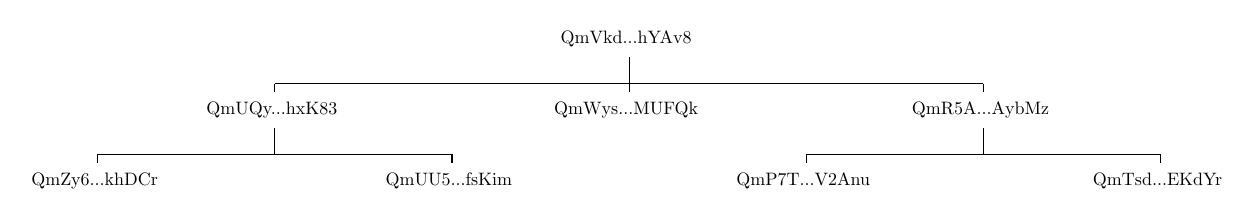
\begin{tikzpicture}[scale = 0.45, every node/.style={scale = 0.65}, every node/.append style={fill = white, rounded corners = 2pt, inner sep = 2pt, align = center}]

  \node at (0, 0) { QmVkd...hYAv8 };

  \draw (0, -0.5) -- (0, -1.5);
  \draw (-10, -1.25) -- (10, -1.25);
  \draw (-10, -1.25) -- (-10, -1.5);
  \draw (10, -1.25) -- (10, -1.5);

  \node at (-10, -2) { QmUQy...hxK83 };
  \node at (0, -2) { QmWys...MUFQk };
  \node at (10, -2) { QmR5A...AybMz };

  \draw (-10, -2.5) -- (-10, -3.25);
  \draw (-15, -3.25) -- (-5, -3.25);
  \draw (-15, -3.25) -- (-15, -3.5);
  \draw (-5, -3.25) -- (-5, -3.5);

  \draw (10, -2.5) -- (10, -3.25);
  \draw (15, -3.25) -- (5, -3.25);
  \draw (15, -3.25) -- (15, -3.5);
  \draw (5, -3.25) -- (5, -3.5);

  \node at (-15, -4) { QmZy6...khDCr };
  \node at (-5, -4) { QmUU5...fsKim };

  \node at (5, -4) { QmP7T...V2Anu };
  \node at (15, -4) { QmTsd...EKdYr };

  \end{tikzpicture}
  \caption{
    Example merkle tree
  }
  \label{fig:example_merkle_tree}
\end{figure}
